\section{Analyse der Ist-Zustand der Barrierefreiheit der Desktopanwendungen}
\unsure{Interne Informationen über die AKG-Software}

\subsection{Barrierefreiheit in der Software-Entwicklung}
Blinde Menschen können keine Computermaus bedienen, d.h. dass die Software komplett per Tastatur bedienbar sein soll. Ein weiterer Grund, wieso Softwareunternehmen sich ebenfalls um digitale Barrierefreiheit kümmern sollten. Es ist eine harte Anforderung an Softwareentwickler, da es bezüglich des erwähnten Beispiels immer üblich war, die Software per Maus zu bedienen. Davon profitieren aber in dem Fall nicht nur Menschen mit Behinderungen. Funktioniert die Maus nicht mehr, so kann die Arbeit mit der Tastatur weitergehen. Programme, die eine Vorlesesoftware anbieten, können nur dann die graphische Oberfläche vorlesen, wenn sie mit Texten beschrieben wurde. Sogar Bilder sind davon betroffen. Ist die Oberfläche nicht gut beschriftet, so kann ein blinder Mensch oder auch Menschen mit Sehschwierigkeiten nichts erkennen. Für Menschen mit Seheinschränkungen ist beispielsweise ein Textcursor, der lediglich als senkrechter Strich im Eingabefeld dargestellt ist, nur schwer zu erkennen. Tastenkombinationen sind auch Barrieren, die für Menschen, die behinderungsbedingt nur eine Hand für das Bedienen der Software einsetzen können, die man durch die Individualisierbarkeit dieser Tastenkombinationen vermeiden kann. Individualisierbarkeit ist auch ein Begriff für Menschen mit Farbfehlsichtigkeit. Softwareunternehmen sollten die Möglichkeit anbieten, die Farben innerhalb der Software zu ändern. Da nicht jedes Unternehmen ihre Software auf digitale Barrierefreiheit testet, haben Menschen mit Behinderungen sehr geringe Auswahlmöglichkeiten.\footnote{PC Welt von IDG \cite{PcWelt}}

\subsubsection{Barrierefreiheit und Behindertengerecht}
\label{subsec:Barrierefreiheit und Behindertengerecht}

Häufig wird das Thema Barrierefreiheit so verstanden, dass es nur bestimmte Zielgruppen betrefft. Der Grund dafür ist, dass das Thema häufig mit Erkrankungen oder Unfällen verbunden wird, die einer offiziellen ärztlichen Diagnose bedürfen. In der Tat haben viel mehr Menschen ein Bedürfnis nach barrierefreier Software, als es ihnen selbst Bewusst ist. In diesem Zusammenhang stellt sich unter anderem die Frage: Warum jeden digitale Barrierefreiheit braucht. Oftmals könnten Situationen dem einen einschränken, diese Situationen fordern barrierefreien Zugang. Was dem einen nach dem letzten Satz sofort einfällt, sind Menschen mit Behinderungen, jedoch ist die Rede hier von jeder Einschränkung, selber wenn sie nicht als Behinderung bezeichnet ist. Die \cref{fig:Beispielhafte Einschränkungen} zeigt diverse Einschränkungen die nicht als Behinderungen zählen.\footnote{Katrin Borecki Usability Engineer, MACH AG \cite{mach}}

\begin{figure}[H]
	\centering
	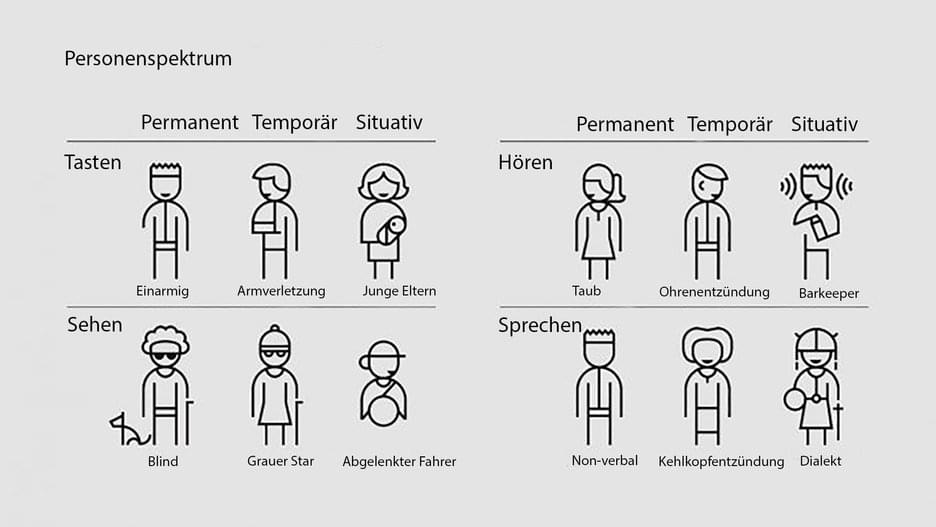
\includegraphics[width=1.0\textwidth]{Barrierefreiheit_personenspektrum}
	\caption[Personen mit verschiedenen Einschränkungen: Permanent, temporär und situativ]{Personen mit verschiedenen Einschränkungen: Permanent, temporär und situativ
	 \cite{mach}}
	\label{fig:Beispielhafte Einschränkungen}
\end{figure}

\subsubsection{Konformitätsstufen anhand der \ac{WCAG}}
\label{subsubsec: Konformitätsstufen}
Nach den Richtlinien der \ac{WCAG} für Barrierefreiheit unterscheidet sich die Umsetzung der Anforderungen an barrierefreie Software in verschiedene Niveaus, die in drei Konformitätsstufen abgestuft sind. Diese sind:

\begin{description}
	\item [Konformitätsstufen A:] Die minimale Konformitätsstufe. Es ist ein Muss, da Menschen sonst die Inhalte nicht wahrnehmen und bedienen können. Wenn
	Erfolgskriterien der Konformitätsstufe A verletzt werden, dann ist mindestens eine Nutzergruppe von der Nutzung ausgeschlossen.\footnote{Hochschule für Technik und Wirtschaft Dresden \cite{HV}}
	
	\item [Konformitätsstufen AA:] Sie ist in Europa und in Deutschland für öffentliche Stellen vorgegeben. Für eine Konformität auf dieser Stufe 
	müssen all Erfolgskriterien der Stufe \textbf{A} und der Stufe \textbf{AA} erfüllt werden. Sind die Erfolgskriterien dieser Stufe nicht umsetzbar, so
	müssen Alternativen dieser Erfolgskriterien
	zur Verfügung gestellt werden. Diese Stufe kann als angestrebte Norm bezeichnet werden, da Menschen sonst die Inhalte nur schwer wahrnehmen und bedienen können.\footnote{Hochschule für Technik und Wirtschaft Dresden \cite{HV}}
	
	\item [Konformitätsstufen AAA:] Um auf diese Stufe zu kommen, müssen zuerst die ersten zwei Stufen \textbf{A} und \textbf{AA} erfüllt werden. "`Kein 
	Webauftritt wird jemals realistischerweise alle WCAG Erfolgskriterien auch der Konformitätsstufe AAA erfüllen. Nicht einmal die WAI empfiehlt, sich 
	dieses Ziel vorzunehmen. Es wird nicht empfohlen, Konformität auf Stufe AAA als allgemeine Richtlinie für komplette Websites zu fordern, da es bei manchen
	Inhalten nicht möglich ist, alle Erfolgskriterien der Stufe AAA zu erfüllen."'\footnote{Zweiter Blick \cite{ZweiterBlick}}
\end{description}

Zur besseren Vorstellung dieser Konformitätsstufen kann \cref{fig:Konformitätsstufen} \footnote{Hochschule für Technik und Wirtschaft Dresden \cite{HV}} beitragen.

\begin{figure}[H]
	\centering
	\includegraphics[width=1.0\textwidth]{Konformitätsstufen}
	\caption[Konformitätsstufen nach der \ac{BITV} 2.0]{Konformitätsstufen nach der \ac{BITV} 2.0}
	\label{fig:Konformitätsstufen}
\end{figure}

\vspace{2cm}

Es bestehen jedoch Ausnahmen für Technologien, die nicht barrierefrei sind und trotzdem dürfen unter den folgenden Bedingungen eingesetzt:\footnote{Web Content Accessibility Guidelines 2.1 \cite{WCAG2.1}}
\begin{itemize}
	\item Falls die Inhalte parallel in einer barrierefreien Version zur Verfügung gestellt werden können.
	\item Solange die Anforderungen der Barrierefreiheit erfüllt sind, können andere Elemente die Wahrnehmung, Bedienbarkeit oder das Verständnis nicht 
	stören. Solche Elemente sind Nicht-Störende-Elemente genannt.
\end{itemize}

\subsubsection{Normen der \ac{WCAG} 2.0}
Die \ac{WCAG} 2.0 sind der internationale Webstandard des \ac{W3C}s zur barrierefreien Gestaltung von Internetseiten. Ab 23. September 2019 gelten die \ac{WCAG} 2.0 in der Europäischen Union für neue Webseiten und ab 23. September 2020 für bestehende Webseiten. In Deutschland wird seit 2002 die Umsetzung der \ac{WCAG} 2.0 durch die gesetzliche Verankerung in der \ac{BITV} gefördert. Die \ac{WCAG} 2.0 legen Erfolgskriterien fest, um die Konformität zu definieren.\footnote{Web Content Accessibility Guidelines 2.0 \cite{WCAG2.0}}

In dieser Projektarbeit werden nur Richtlinien betrachtet, die einen Einfluss auf die Desktopsoftware haben können. D.h. Richtlinien, die nur z.B. die mobile Nutzung berücksichtigen, werden in dieser Projektarbeit ignoriert. Dasselbe gilt auch in \cref{subsec: Normen der WCAG 2.1}.

Zu den wichtigen Richtlinien zählt:\footnote{Web Content Accessibility Guidelines 2.0 \cite{WCAG2.0}}

\begin{description}
	\item[Richtlinie 1.1 Textalternativen]\hfill
	\begin{itemize}
		\item \textbf{Prinzip:} Wahrnehmbar.
		\item \textbf{Allgemeine Beschreibung:} Für alle Nicht-Text-Inhalte müssen Textalternativen zur Verfügung gestellt werden, damit der Benutzer die
		präsentierte Form der Inhalte nach seinem Bedürfnis ändern kann.
	\end{itemize}
	
	\begin{description}
		\item[Richtlinie 1.1.1 Nicht-Text-Inhalt]\hfill
		\begin{itemize}
			\item \textbf{Konformitätsstufe:} A
			\item \textbf{Beschreibung:} Es müssen Mitteln zum Ersetzen der Nicht-Text-Inhalte dargestellt werden können, so dass dem Benutzer die
			Nicht-Text-Inhalte nicht verhindern. Beispielsweise die Anpassung der Schriftgröße, die Verwendung von Symbolen oder Brailleschrift sowie den Text 
			in einer einfachere Sprache verwandeln zu können. Das sind alle Mitteln, die zur Textalternativen zählen.
			Nichtsdestotrotz gibt es dafür Ausnahmen: Steuerelemente oder Eingaben durch den Benutzer, denn diese einen Namen haben, der den Zweck des Element
			beschreibt. Außerdem sind Tests und Übungen von dieser Richtlinie ausgenommen, da einen alternativen Text eine deskriptive Identifizierung
			des Tests oder der Übung bereitstellt und damit entfällt den Sinn des Tests bzw. der Übung. Wenn es um die Vermittlung/Schaffung bestimmter
			Sinneserfahrungen handelt, kann das Nicht-Text-Element ohne Textalternativen präsentiert werden. Darüber hinaus sind \ac{CAPTCHA} vom Regel ausgenommen,
			denn es darum geht, vom Benutzer eine Bestätigung zu verlangen, dass überhaupt eine Person und kein Computer auf den Inhalt zugreift. Allerdings gibt
			es statt die Textalternativen für das Ersetzen von \ac{CAPTCHA}s andere Ausgabeformen, die die sensorischen Wahrnehmung nutzen. Unsichtbare Elemente
			oder reine Dekoration, die ausschließlich für visuelle Formatierung verwendet wird, müssen keine Textalternativen haben, dennoch müssen
			sie so implementiert werden, dass sie von assistierender Technik ignoriert werden können.
		\end{itemize}
	\end{description}
	
	\item[Richtlinie 1.2 Zeitbasierte Medien]\hfill
	\begin{itemize}
		\item \textbf{Prinzip:} Wahrnehmbar.
		\item \textbf{Allgemeine Beschreibung:} Es geht darum, dass alternativen zu den Zeitbasierte Medien zur Verfügung gestellt werden müssen. Davon ausgenommen sind 
		Medien, die Alternative zum Text sind.
	\end{itemize}
	
	\begin{description}
		\item[Richtlinie 1.2.1 Reine Audio- und Videoinhalte (aufgezeichnet)]\hfill
		\begin{itemize}
			\item \textbf{Konformitätsstufe:} A
			\item \textbf{Beschreibung:} Eine Alternative für reine aufgezeichnete Audio- und Videoinhalte, die äquivalente Informationen 
			liefert, muss bereitgestellt werden.
		\end{itemize}
			
		\item[Richtlinie 1.2.2 Untertitel (aufgezeichnet)]\hfill
		\begin{itemize}
			\item \textbf{Konformitätsstufe:} A
			\item \textbf{Beschreibung:} Für alle aufgezeichnete Audioinhalte in synchronisierten Medien müssen Untertiteln bereitgestellt werden.
		\end{itemize}
			
		\item[Richtlinie 1.2.3 Audiodeskription (aufgezeichnet)]\hfill
		\begin{itemize}
			\item \textbf{Konformitätsstufe:} A
			\item \textbf{Beschreibung:} Es muss für synchronisierten Medien eine Audiodeskription des aufgezeichneten Videoinhalts oder andere 
			Medienalternativen zur Verfügung gestellt werden.
		\end{itemize}
			
		\item[Richtlinie 1.2.4 Untertitel (Live)]\hfill
		\begin{itemize}
			\item \textbf{Konformitätsstufe:} AA
			\item \textbf{Beschreibung:} Für alle Live-Audioinhalte muss Untertitel bereitgestellt werden.
		\end{itemize}
			
		\item[Richtlinie 1.2.5 Audiodeskription (aufgezeichnet)]\hfill
		\begin{itemize}
			\item \textbf{Konformitätsstufe:} AA
			\item \textbf{Beschreibung:} Alle aufgezeichnete Videoinhalte in synchronisierten Medien müssen eine Audiodeskription haben.
		\end{itemize}
			
		\item[Richtlinie 1.2.6 Gebärdensprache (aufgezeichnet)]\hfill
		\begin{itemize}
			\item \textbf{Konformitätsstufe:} AAA
			\item \textbf{Beschreibung:} Für alle aufgezeichnete Videoinhalte in in synchronisierten Medien muss eine Übersetzung in die Gebärdensprache zur 
			Verfügung gestellt wird.
		\end{itemize}
			
		\item[Richtlinie 1.2.7 Erweiterte Audiodeskription (aufgezeichnet)]\hfill
		\begin{itemize}
			\item \textbf{Konformitätsstufe:} AAA
			\item \textbf{Beschreibung:} Sind die Pausen im Haupt-Audio für eine Audiodeskription nicht ausreichend, um den Sinn des Inhaltes zu vermitteln oder 
			wichtige Details zu beschreiben, dann sind für alle aufgezeichnete Videoinhalte in synchronisierten Medien eine erweiterte 
			Audiodeskription bereitzustellen.
		\end{itemize}
			
		\item[Richtlinie 1.2.8 Medienalternative (aufgezeichnet)]\hfill
		\begin{itemize}
			\item \textbf{Konformitätsstufe:} AAA
			\item \textbf{Beschreibung:} Für alle aufgezeichneten synchronisierten Medien muss eine Alternative für zeitbasierte Medien bereitgestellt werden.
		\end{itemize}
			
		\item[Richtlinie 1.2.9 Reiner Audioinhalt (Live)]\hfill
		\begin{itemize}
			\item \textbf{Konformitätsstufe:} AAA
			\item \textbf{Beschreibung:} Eine Alternative für zeitbasierte Medien muss zur Verfügung gestellt werden, die äquivalente Informationen 
			für live übertragene reine Audioinhalte anbietet.
		\end{itemize}
			
	\end{description}

	\item[Richtlinie 1.3 Anpassbar]\hfill
	\begin{itemize}
		\item \textbf{Prinzip:} Wahrnehmbar.
		\item \textbf{Allgemeine Beschreibung:} Das Präsentieren der Inhalte muss auf verschiedene Arten ohne Verlust von Informationen oder 
		Struktur dargestellt werden können.
	\end{itemize}
	
	\begin{description}
		\item[Richtlinie 1.3.1 Informationen und Beziehungen]\hfill
		\begin{itemize}
			\item \textbf{Konformitätsstufe:} A
			\item \textbf{Beschreibung:} Falls Informationen, Struktur und Beziehungen über die Darstellung vermittelt werden, müssen diese durch Software bestimmt 
			werden oder in Textform bereitgestellt.
		\end{itemize}
			
		\item[Richtlinie 1.3.2 Bedeutungstragende Reihenfolge]\hfill
		\begin{itemize}
			\item \textbf{Konformitätsstufe:} A
			\item \textbf{Beschreibung:} Wirkt sich die Reihenfolge der Inhalte auf die Bedeutung der Inhalte aus, so muss die korrekte Leseabfolge durch Software 
			bestimmt werden können. Mit einer korrekten Leseabfolge ist gemeint, dass die Reihenfolge der Inhalte deren Bedeutung nicht verändert.
		\end{itemize}
			
		\item[Richtlinie 1.3.3 Sensorische Eigenschaften]\hfill
		\begin{itemize}
			\item \textbf{Konformitätsstufe:} A
			\item \textbf{Beschreibung:} Falls es Anweisungen gibt, die für das Verständnis und die Bedienung der Inhalte zur Verfügung stehen, müssen diese 
			nicht nur von sensorische Eigenschaften der Komponenten abhängig sein, wie z.B. die visuelle Position oder die Größe des Elements.
		\end{itemize}
	\end{description}

	\item[Richtlinie 1.4 Unterscheidbar]\hfill
	\begin{itemize}
		\item \textbf{Prinzip:} Wahrnehmbar.
		\item \textbf{Allgemeine Beschreibung:} Den Benutzern muss es leichter fallen, Inhalt zu sehen und zu hören.
	\end{itemize}
	
	\begin{description}
		\item[Richtlinie 1.4.1 Benutzung von Farbe]\hfill
		\begin{itemize}
			\item \textbf{Konformitätsstufe:} A
			\item \textbf{Beschreibung:} Um Inhalte zu unterscheiden oder Informationen zu vermitteln, darf die Farben nicht das einzige Mittel benutzt werden.
		\end{itemize}
		
		\item[Richtlinie 1.4.2 Audio-Steuerelement]\hfill
		\begin{itemize}
			\item \textbf{Konformitätsstufe:} A
			\item \textbf{Beschreibung:} Wird einen Audioinhalt auf der Webseite für mehr als 3 Sekunden abgespielt, dann wird die Möglichkeit angeboten, dass der 
			Benutzer dieses Element steuert. Entweder kann der Benutzer das Audioelement pausieren oder die Lautstärke des Audioelements unabhängig von der 
			allgemeinen Systemlautstärke regeln.
		\end{itemize}
		
		\item[Richtlinie 1.4.3 Kontrast (Minimum)]\hfill
		\begin{itemize}
			\item \textbf{Konformitätsstufe:} AA
			\item \textbf{Beschreibung:} Das Kontrastverhältnis von Text und Bilder, die Text enthalten, muss mindestens 4,5 zu 1 (4,5:1) sein. Falls der Text größer 
			als 14pt, dann muss das Kontrastverhältnis davon mind. 3 zu 1 (3:1) sein. Ausgenommen sind die reinen dekorativen Inhalte (Die keine Informationen liefern).
		\end{itemize}
		
		\item[Richtlinie 1.4.4 Textgröße ändern]\hfill
		\begin{itemize}
			\item \textbf{Konformitätsstufe:} AA
			\item \textbf{Beschreibung:} Die Textgröße muss bis zu 200 Prozent ohne Verlust von Inhalte geändert werden können. Davon ausgenommen sind die 
			Untertiteln und Bilder eines Textes.
		\end{itemize}
		
		\item[Richtlinie 1.4.5 Bilder eines Textes]\hfill
		\begin{itemize}
			\item \textbf{Konformitätsstufe:} AA
			\item \textbf{Beschreibung:} Falls mit der Darstellung von Bilder eines Textes Informationen verloren gehen können, dann wird Text statt Bilder eines Textes 
			benutzt werden.
		\end{itemize}
		
		\item[Richtlinie 1.4.6 Kontrast (erhöht)]\hfill
		\begin{itemize}
			\item \textbf{Konformitätsstufe:} AAA
			\item \textbf{Beschreibung:} Das Kontrastverhältnis von Text und Bilder eines Textes muss mindestens 7 zu 1 sein. Für größere Texte (Größer als 14pt)bzw. 
			Bilder eines Textes ist das Kontrastverhältnis mindestens 4,5 zu 1. Analog zur Richtlinie 1.4.3 sind die reinen dekorativen Inhalte von 
			der Regel ausgenommen.
		\end{itemize}
		
		\item[Richtlinie 1.4.7 Leiser oder kein Hintergrund-Audioinhalt]\hfill
		\begin{itemize}
			\item \textbf{Konformitätsstufe:} AAA
			\item \textbf{Beschreibung:} Aufgezeichneter Audioinhalt, der Sprache im Vordergrund hat, kein Audio-CAPTCHA oder Audio-Logo und kein musikalischer Ausdruck
			wie z.B. Singen ist, muss abgeschaltet werden können oder gar keine Hintergrundgeräusche enthält, oder dass die Hintergrundgeräusche mindestens 20 Dezibel 
			leiser als der Sprachinhalt im Vordergrund sind.
		\end{itemize}
		
		\item[Richtlinie 1.4.8 Visuelle Präsentation]\hfill
		\begin{itemize}
			\item \textbf{Konformitätsstufe:} AAA
			\item \textbf{Beschreibung:} Für die Darstellung von Textblöcken gilt:
			\begin{itemize}
				\item Vorder- und Hintergrundfarben können geändert werden.
				\item Text ist nicht im Blocksatz ausgerichtet.
				\item Die Breite beträgt nicht mehr als 80 Zeichen.
				\item Innerhalb von Paragraphen ist der der Zeilenabstand mindestens 1,5-fach und zwischen Paragraphen mindestens 1,5-fach so 
				groß wie der Zeilenabstand.
				\item Die Textgröße kann ohne zusätzliche Technik bis auf 200\% skaliert werden und das ohne, dass der Leser dafür scrollen muss.
			\end{itemize}
		\end{itemize}
		
		\item[Richtlinie 1.4.9 Bilder eines Textes (keine Ausnahme)]\hfill
		\begin{itemize}
			\item \textbf{Konformitätsstufe:} AAA
			\item \textbf{Beschreibung:} Bilder eines Textes können nur dann benutzt, wenn sie entweder rein dekorativ sind oder wenn die Vermittlung von bestimmten 
			 Informationen anders nicht geht. Ein Beispiel dafür ist der Text in einem Logo.
		\end{itemize}
	\end{description}
	
	\item[Richtlinie 2.1 Per Tastatur zugänglich]\hfill
	\begin{itemize}
		\item \textbf{Prinzip:} Bedienbar.
		\item \textbf{Allgemeine Beschreibung:} Alle Funktionalitäten sind per Tastatur erreichbar sein.
	\end{itemize}
	
	\begin{description}
		\item[Richtlinie 2.1.1 Tastatur]\hfill
		\begin{itemize}
			\item \textbf{Konformitätsstufe:} A
			\item \textbf{Beschreibung:} Durch eine Tastaturschnittstelle müssen alle möglichen Funktionalitäten bedienbar sein. Ohne dass eine bestimmte 
			Zeiteinteilung für einzelne Tastenanschläge erforderlich ist. Eingabetechniken sind in diesem Zusammenhang nicht gemeint.
		\end{itemize}
		
		\item[Richtlinie 2.1.2 Keine Tastaturfalle]\hfill
		\begin{itemize}
			\item \textbf{Konformitätsstufe:} A
			\item \textbf{Beschreibung:} Anhand der Tastaturschnittstelle muss der Tastaturfokus von einem Bestandteil zum anderen Bewegt werden können. Außerdem wenn 
			die üblichen Methoden zum Aussteigen von einem Bestandteil abweicht, wird der Benutzer darüber informiert.
		\end{itemize}
		
		\item[Richtlinie 2.1.3 Tastatur (keine Ausnahme)]\hfill
		\begin{itemize}
			\item \textbf{Konformitätsstufe:} AAA
			\item \textbf{Beschreibung:} Analog zur Richtlinie 2.1.1 nur ohne Ausnahmen.
		\end{itemize}
	\end{description}
	
	\item[Richtlinie 2.2 Ausreichend Zeit]\hfill
	\begin{itemize}
		\item \textbf{Prinzip:} Bedienbar.
		\item \textbf{Allgemeine Beschreibung:} Der Benutzer erhält genügend Zeit, um Inhalte zu lesen und benutzen.
	\end{itemize}
	
	\begin{description}
		\item[Richtlinie 2.2.1 Zeiteinteilung anpassbar]\hfill
		\begin{itemize}
			\item \textbf{Konformitätsstufe:} A
			\item \textbf{Beschreibung:} Falls es zeitlich begrenzte Inhalte gibt, dann gilt für diesen Inhalt:
			\begin{itemize}
				\item Abschalten \& Anpassen und das bevor der Benutzer auf diesen Inhalt trifft.
				\item Ausweiten der zeitlichen Begrenzung, bevor sie abläuft und zwar so, dass der Benutzer vor mind. 20 Sekunden gewarnt wird. Der Benutzer muss 
				dementsprechend informiert werden, wie er die zeitlichen Begrenzung ausweitet.
			\end{itemize}
			Es gelten für diese Richtlinie folgende Ausnahmen: Wenn es beispielsweise um Echtzeit-Inhalt handelt wie eine Auktion oder wenn die Ausweitung 
			der zeitlichen Begrenzung den Inhalt ungültig macht. Wenn die zeitliche Begrenzung mehr als 20 Stunden dauert, dann gilt die nicht mehr.
		\end{itemize}
		
		\item[Richtlinie 2.2.2 Pausieren, beenden, ausblenden]\hfill
		\begin{itemize}
			\item \textbf{Konformitätsstufe:} A
			\item \textbf{Beschreibung:} Für Inhalte, die sich automatisch bewegen, aktualisieren, scrollen und blinken (Wechseln zwischen mehreren Zuständen um dem 
			Benutzer aufmerksam zu machen), muss der Benutzer sie steuern können, indem er sie pausieren, beenden und ausblenden können, es sei denn, dass eine der 
			erwähnten Aktionen ein Teil einer Handlung ist, ohne ihn Informationen verloren gehen können.
		\end{itemize}
		
		\item[Richtlinie 2.2.3 Keine Zeiteinteilung]\hfill
		\begin{itemize}
			\item \textbf{Konformitätsstufe:} AAA
			\item \textbf{Beschreibung:} Gar keine Keine zeitlich begrenzte Inhalte, es sei denn, dass es sich um Echtzeit-Ereignisse (Eine Auktion) oder  
			synchronisierten Medien handelt.
		\end{itemize}
		
		\item[Richtlinie 2.2.4 Unterbrechungen]\hfill
		\begin{itemize}
			\item \textbf{Konformitätsstufe:} AAA
			\item \textbf{Beschreibung:} Der Benutzer kann jede Unterbrechungen aufschieben oder unterdrücken, es sei denn, dass es sich um einen Notfall handelt.
		\end{itemize}
		
		\item[Richtlinie 2.2.5 Erneute Authentifizierung]\hfill
		\begin{itemize}
			\item \textbf{Konformitätsstufe:} AAA
			\item \textbf{Beschreibung:} Es geht darum, dass der Benutzer ohne Datenverlust nach der erneuten Authentifizierung (Wenn die Sitzung abläuft) 
			fortfahren kann.
		\end{itemize}
	\end{description}
	
	\item [Richtlinie 2.3 Anfälle]\hfill
	\begin{itemize}
		\item \textbf{Prinzip:} Bedienbar.
		\item \textbf{Allgemeine Beschreibung:} Die Gestaltung der Inhalte darf nicht zu Anfällen führen.
	\end{itemize}
	
	\begin{description}
		\item[Richtlinie 2.3.1 Grenzwert von dreimaligem Blitzen oder weniger]\hfill
		\begin{itemize}
			\item \textbf{Konformitätsstufe:} A
			\item \textbf{Beschreibung:} Webseiten dürfen keine Elemente/Inhalte haben, die mehr als dreimal in einem beliebigen, eine Sekunde dauernden Zeitraum 
			blitzen. Es gilt für dieses Richtlinie eine Ausnahme und zwar wenn der Blitz unterhalb der allgemeinen Grenzwerte zu Blitzen und roten Blitzen 
			(Siehe \nameref{subsec: Anlage1}).
		\end{itemize}
		
		\item[Richtlinie 2.3.2 Drei Blitze]\hfill
		\begin{itemize}
			\item \textbf{Konformitätsstufe:} AAA
			\item \textbf{Beschreibung:} Analog zur Richtlinie 2.3.1 nur ohne Ausnahmen.
		\end{itemize}
	\end{description}
	
	\item[Richtlinie 2.4 Navigierbar]\hfill
	\begin{itemize}
		\item \textbf{Prinzip:} Bedienbar.
		\item \textbf{Allgemeine Beschreibung:} Es werden Mittels dem Benutzer bereitgestellt, um Inhalte zu finden und zu bestimmen, wo sie sind.
	\end{itemize}
	
	\begin{description}
		\item[Richtlinie 2.4.1 Blöcke umgehen]\hfill
		\begin{itemize}
			\item \textbf{Konformitätsstufe:} A
			\item \textbf{Beschreibung:} Gibt es Inhaltsblöcke, die sich auf verschiedenen Webseiten wiederholt werden, dann werden Mittels zur Verfügung 
			gestellt werden, um diese Inhaltsblöcke umzugehen.		
		\end{itemize}
		
		\item[Richtlinie 2.4.2 Seite mit Titel versehen]\hfill
		\begin{itemize}
			\item \textbf{Konformitätsstufe:} A
			\item \textbf{Beschreibung:} Jede Webseite bekommt einen Titel, der beschreibt, worum es sich in der Webseite handelt.
		\end{itemize}
		
		\item[Richtlinie 2.4.3 Fokus-Reihenfolge]\hfill
		\begin{itemize}
			\item \textbf{Konformitätsstufe:} A
			\item \textbf{Beschreibung:} Kann die Webseite der Reihe nach navigiert werden und spielt die Reihenfolge der Navigation für die Bedeutung eine 
			Rolle, dann erhalten fokussierbare Komponenten den Fokus in einer Reihenfolge, in der die Bedeutung und die Bedienbarkeit erhalten bleiben.
		\end{itemize}
		
		\item[Richtlinie 2.4.4 Linkzweck (im Kontext)]\hfill
		\begin{itemize}
			\item \textbf{Konformitätsstufe:} A
			\item \textbf{Beschreibung:} Der Linktext muss den Zweck des linkes allein beschreiben oder durch den Linktext mit zusätzlichen 
			Informationen, die durch Software bestimmt werden können. Eine Ausnahme gilt, wenn die Bedeutung des Links für den Benutzer mehrdeutig wäre.
		\end{itemize}
		
		\item[Richtlinie 2.4.5 Verschiedene Methoden]\hfill
		\begin{itemize}
			\item \textbf{Konformitätsstufe:} AA
			\item \textbf{Beschreibung:} Es werden Methoden bereitgestellt werden, um eine Webseite innerhalb einer Sammlung von Webseiten, die einem 
			gemeinsamen Zweck dienen, zu finden, es sei denn, dass die Webseite das Ergebnis oder ein Schritt eines Prozesses ist.
		\end{itemize}
		
		\item[Richtlinie 2.4.6 Überschriften und Beschriftungen (Labels)]\hfill
		\begin{itemize}
			\item \textbf{Konformitätsstufe:} AA
			\item \textbf{Beschreibung:} Überschriften und Labels müssen entweder ein Thema oder einen Zweck beschreiben.
		\end{itemize}
		
		\item[Richtlinie 2.4.7 Fokus sichtbar]\hfill
		\begin{itemize}
			\item \textbf{Konformitätsstufe:} AA
			\item \textbf{Beschreibung:} Für jede Benutzerschnittstelle, die durch die Tastatur bedienbar ist, gilt: Sie muss über einen Bedienmodus
			verfügen, der dem Tastaturfokus sichtbar macht.
		\end{itemize}
		
		\item[Richtlinie 2.4.8 Position]\hfill
		\begin{itemize}
			\item \textbf{Konformitätsstufe:} AAA
			\item \textbf{Beschreibung:} Es werden Informationen über die Position des Benutzers (Wo sich der Benutzer befindet, falls es um eine 
			Sammlung von Webseiten geht) zur Verfügung gestellt werden.
		\end{itemize}
		
		\item[Richtlinie 2.4.9 Linkzweck (reiner Link)]\hfill
		\begin{itemize}
			\item \textbf{Konformitätsstufe:} AAA
			\item \textbf{Beschreibung:} Der Linktext beschreibt allein den Zweck des Linkes, es sei denn, die Bedeutung des Links für den Benutzer 
			mehrdeutig wäre.
		\end{itemize}
		
		\item[Richtlinie 2.4.10 Abschnittsüberschriften]\hfill
		\begin{itemize}
			\item \textbf{Konformitätsstufe:} AAA
			\item \textbf{Beschreibung:} Die Überschriften der Abschnitte werden verwenden, um den Inhalt zu strukturieren.
		\end{itemize}
	\end{description}	
	
	\item[Richtlinie 3.1 Lesbar]\hfill
	\begin{itemize}
		\item \textbf{Prinzip:} Verständlich.
		\item \textbf{Allgemeine Beschreibung:} Alle Inhalte müssen lesbar und verständlich sein.
	\end{itemize}
	
	\begin{description}
		\item[Richtlinie 3.1.1 Sprache der Seite]\hfill
		\begin{itemize}
			\item \textbf{Konformitätsstufe:} A
			\item \textbf{Beschreibung:} Die voreingestellte menschliche Sprache (Jede Sprache, die gesprochen, geschrieben oder gebärdet werden kann) jeder Webseite muss 
			durch Software bestimmt werden können.
		\end{itemize}
		
		\item[Richtlinie 3.1.2 Sprache von Teilen]\hfill
		\begin{itemize}
			\item \textbf{Konformitätsstufe:} AA
			\item \textbf{Beschreibung:} "`Die menschliche Sprache jedes Abschnitts oder jedes Satzes im Inhalt kann durch Software bestimmt werden außer
			bei Eigennamen, technischen Fachbegriffen, Wörtern einer unklaren Sprache und Wörtern oder Wendungen, die Teil des Jargons des direkt 
			umliegenden Textes geworden sind"'.\footnote{Web Content Accessibility Guidelines 2.0 \cite{WCAG2.0}}
		\end{itemize}
		
		\item[Richtlinie 3.1.3 Ungewöhnliche Wörter]\hfill
		\begin{itemize}
			\item \textbf{Konformitätsstufe:} AAA
			\item \textbf{Beschreibung:} Spezielle Definitionen von Wörtern und Wendungen müssen erkannt werden können. Diese können Wörter, die auf ungewöhnlicher 
			Weise benutzt werden.
		\end{itemize}
		
		\item[Richtlinie 3.1.4 Abkürzungen]\hfill
		\begin{itemize}
			\item \textbf{Konformitätsstufe:} AAA
			\item \textbf{Beschreibung:} Die Bedeutung oder die ausgeschriebene Form von Abkürzungen wird durch ein Mechanismus erkannt.
		\end{itemize}
		
		\item[Richtlinie 3.1.5 Leseniveau]\hfill
		\begin{itemize}
			\item \textbf{Konformitätsstufe:} AAA
			\item \textbf{Beschreibung:} Verlangt der Text bestimmte Lesefähigkeiten, die über das Niveau der niedrigen sekundären Schulbildung hinausgehen (Die 
			Phase nach der Beendung der ersten sechs Schuljahre), dann wird andere Version des Textes in einer einfacheren Sprache zur Verfügung gestellt werden.
		\end{itemize}
		
		\item[Richtlinie 3.1.6 Aussprache]\hfill
		\begin{itemize}
			\item \textbf{Konformitätsstufe:} AAA
			\item \textbf{Beschreibung:} 
		\end{itemize}
	\end{description}

	\item[Richtlinie 3.2 Vorhersehbar]\hfill
	\begin{itemize}
		\item \textbf{Prinzip:} Verständlich.
		\item \textbf{Allgemeine Beschreibung:} 
	\end{itemize}
	
	\begin{description}
		\item[Richtlinie ]\hfill
		\begin{itemize}
			\item \textbf{Konformitätsstufe:}
			\item \textbf{Beschreibung:}
		\end{itemize}
	\end{description}

	\item[Richtlinie 3.3 Hilfestellung bei der Eingabe]\hfill
	\begin{itemize}
		\item \textbf{Prinzip:} Verständlich.
		\item \textbf{Allgemeine Beschreibung:} 
	\end{itemize}
	
	\begin{description}
		\item[Richtlinie ]\hfill
		\begin{itemize}
			\item \textbf{Konformitätsstufe:}
			\item \textbf{Beschreibung:}
		\end{itemize}
	\end{description}

	\item[Richtlinie 4.1 Kompatibel]\hfill
	\begin{itemize}
		\item \textbf{Prinzip:} Robust.
		\item \textbf{Allgemeine Beschreibung:} Ziel ist das Maximieren der Kompatibilität von den aktuellen und zukünftigen Benutzeragenten, 
		einschließlich assistierender Techniken. Es muss sichergestellt werden, dass Autoren nichts tun, was assistierende Techniken brechen kann bzw. 
		was von den assistierenden Techniken nicht erkannt werden kann.
	\end{itemize}
	
	\begin{description}
		\item[Richtlinie 4.1.1 Syntaxanalyse]\hfill
		\begin{itemize}
			\item \textbf{Konformitätsstufe:} A
			\item \textbf{Beschreibung:} Es gilt für Inhalte, die durch Auszeichnungssprachen implementiert wurden:
			\begin{itemize}
				\item Elemente dieser Inhalte haben Start- und Endtags.
				\item Wenn die Elemente entsprechend ihrer Spezifikationen verschachtelt werden, erhalten sie keine doppelte Attribute und alle ihrer
				 IDs sind einzigartig. Ausgenommen wenn die Spezifikationen diese erlaubt.
				 
			\end{itemize}
		\end{itemize}
		
		\item[Richtlinie 4.1.2 Name, Rolle, Wert]\hfill
		\begin{itemize}
			\item \textbf{Konformitätsstufe:} A
			\item \textbf{Beschreibung:} Alle Bestandteile einer Benutzerschnittstelle müssen durch Software bestimmt werden können. Diese können 
			Namen, Rollen, Zustände, Eigenschaften und Werte, die vom Benutzer festgelegt werden können. Außerdem müssen Benachrichtigung über Änderungen 
			an diesen Elementen dem Benutzer zur Verfügung gestellt werden.
		\end{itemize}
	\end{description}

\end{description}

\subsubsection{Normen der \ac{BITV} 2.0}
Die \ac{BITV} mit der Version 2.0 wurde in Deutschland im September 2011 veröffentlicht. Ihre Ziel ist die Umsetzung barrierefreier Webinhalte in Deutschland.\footnote{Bundesministerium der Justiz und für Verbracuerschutz\cite{BITV}} Bei der \ac{BITV} 2.0 unterscheidet man zwei Bereiche:

\begin{itemize}
	\item Die Umsetzung für Behörden: Zwingend.
	\item Die Umsetzung für private Bereiche: Wünschenswert.
\end{itemize}

Die \ac{BITV} 2.0 basiert zum größten Teil auf den \ac{WCAG} 2.0 der \ac{WAI}. Bei der \ac{BITV} 2.0 sind auch die vier Prinzipien für Barrierefreiheit der \ac{WCAG} 2.0  enthalten, die in \cref{subsec:Prinzipien fuer Barrierefreiheit} erklärt sind. Des weiteren gibt es zwischen den \ac{WCAG} 2.0 und der \ac{BITV} 2.0 Unterschiede:\footnote{Die Barrierefreie-Informationstechnik-Verordnung 2.0 \cite{BITV}}

\begin{itemize}
	\item Die Konformitätsstufen der \ac{WCAG} 2.0, die in \cref{subsubsec: Konformitätsstufen} beschrieben sind. Sie sind in zwei Stufen bei 
	der \ac{BITV} 2.0 unterteilt:
		\begin{itemize}
			\item Stufe I: Sie beinhaltet die Konformitätsstufe A und die Konformitätsstufe AA der \ac{WCAG} 2.0
			\item Stufe II: Sie beinhaltet die Konformitätsstufe AAA der \ac{WCAG} 2.0
		\end{itemize}
	
	\item Bei der \ac{BITV} 2.0 wurde auf Hilfestellungen verzichtet, bei diesen handelt es sich um Erklärungen für die richtige Umsetzung der Kriterien.
	
	\item Das Erfolgskriterium 2.4.8 besitzt bei den \ac{WCAG} 2.0 die Konformitätsstufen AAA und bei der \ac{BITV} die Stufe I. Dieses Erfolgskriterium besagt, dass 
	Mittel zur Verfügung gestellt werden müssen, um Benutzer bei der Navigation zu unterstützen, und um Inhalte zu finden und zu bestimmen.
	
	\item Die \ac{BITV} 2.0 beinhaltet zusätzlich weitere Anforderungen an die Gestaltung von Gebärdensprechfilmen und Texten in leichter Sprache, diese hilft
	z.B. Menschen mit Lern- und geistigen Behinderungen.
\end{itemize}

\subsubsection{Normen der \ac{WCAG} 2.1 als Erweiterung}
\label{subsec: Normen der WCAG 2.1}

Basiert auf der Version \ac{WCAG} 2.0 und ersetzt sie nicht, sondern zählt als Erweiterung. Zu den Richtlinien der \ac{WCAG} 2.0 wurden mit den \ac{WCAG} 2.1 17 neue Kriterien hinzugefügt, die vor allem die mobile Nutzung sowie die Nutzung durch sehbehinderte oder lernbehinderte Personen betreffen.\footnote{Barrierefreies Webdesign \cite{BarrierefreiesWebdesign}}

